\documentclass[]{article}
\usepackage{tikz}

\begin{document}
    \begin{tikzpicture}
        % (0,0)为起点,(30:1)分别为30° r=1 单位缺省时为cm
        \draw (0,0) -- (30:1);
        % 点(1,0)到(2,1)
        \draw (1,0) -- (2,1);
        % 给(0,1)点命名,以后就可以使用(S)作为点的位置
        \coordinate (S) at (0,1);
        \draw (S) -- (1,1);
    \end{tikzpicture}
    \begin{tikzpicture}
        \coordinate (S) at (2,2);
        \draw[gray] (-1,2) -- (S);
        \draw[gray] (2,-1) -- (S);
        % 坐标的表示形式还包括“垂足”形式
        \draw[red] (0,0) -- (0,0 -| S);
        \draw[blue] (0,0) -- (0,0 |- S);
    \end{tikzpicture}
    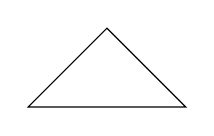
\begin{tikzpicture}
        \draw (0,0) -- (1,1)
        -- (2,0) -- cycle;
        % 使用cycle 令路径回到起点,生成闭合的路径
    \end{tikzpicture}
    % 网格、函数图像,网格可用step 参数控制网格大小,函数图像用domain 参数控制定义域:
    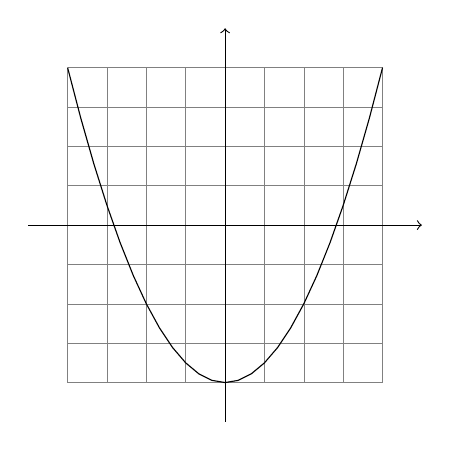
\begin{tikzpicture}
        \draw[help lines,step=0.5]
        (-2,-2) grid (2,2);
        \draw[->] (-2.5,0) -- (2.5,0);
        \draw[->] (0,-2.5) -- (0,2.5);
        \draw[domain=-2:2]
        plot(\x,{\x*\x -2});
    \end{tikzpicture}
    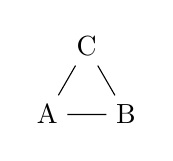
\begin{tikzpicture}
        \node (A) at (0,0) {A};
        \node (B) at (1,0) {B};
        \node (C) at (60:1) {C};
        \draw (A) -- (B) -- (C) -- (A);
    \end{tikzpicture}
    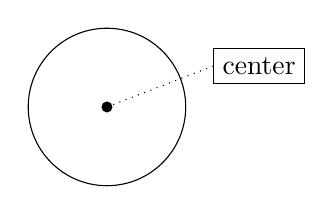
\begin{tikzpicture}
        \draw (0,0) circle[radius=1];
        \fill (0,0) circle[radius=2pt];
        \node[draw] (P) at (15:2) {center};
        \draw[dotted] (0,0) -- (P.west);
    \end{tikzpicture}
    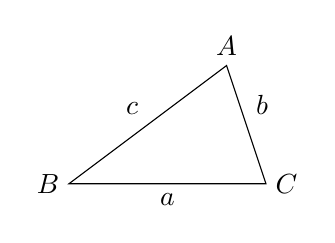
\begin{tikzpicture}
        \draw (2,1.5) node[above] {$A$}
        -- node[above left] {$c$}
        (0,0) node[left] {$B$}
        -- node[below] {$a$}
        (2.5,0) node[right] {$C$}
        -- node[above right] {$b$}
        cycle;
    \end{tikzpicture}
    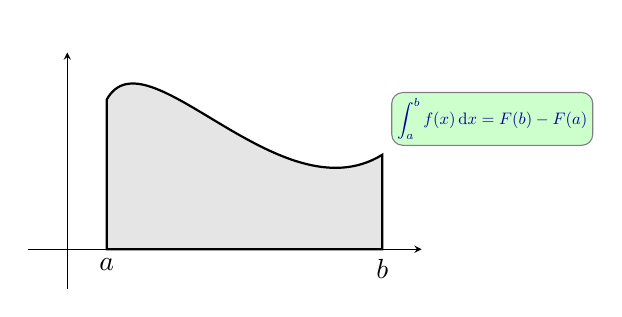
\begin{tikzpicture}
        \draw[-stealth,line width=0.2pt] (-0.5,0) -- (4.5,0);
        \draw[-stealth,line width=0.2pt] (0,-0.5) -- (0,2.5);
        \coordinate (a) at (0.5,1.9);
        \coordinate (b) at (4,1.2);
        \coordinate[label=below:$a$] (a0) at (a |- 0,0);
        \coordinate[label=below:$b$] (b0) at (b |- 0,0);
        \filldraw[fill=gray!20,draw,thick]
        (a0) -- (a) .. controls (1,2.8) and (2.7,0.4) .. (b) -- (b0) -- cycle;
        \node[above right,outer sep=0.2cm, rounded corners,
        fill=green!20,draw=gray,text=blue!60!black,scale=0.6]
        at (b) {$\displaystyle \int_a^b {f(x)\,\mathrm{d}x} = F(b) - F(a)$};
    \end{tikzpicture}
    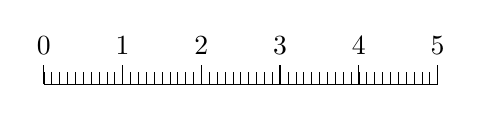
\begin{tikzpicture}
        \draw (0,0)--(5,0);
        \foreach \i in {0.0,0.1,...,5.0}
        {\draw[very thin]
        (\i,0)--(\i,0.15);}
        \foreach \I in {0,1,2,3,4,5}
        {\draw (\I,0)--(\I,0.25)
        node[above] {\I};}
    \end{tikzpicture}
\end{document}